\documentclass{ximera}
% \handouttrue
%\graphicspath{  %% When looking for images,
{./}            %% look here first,
{./pictures/}   %% then look for a pictures folder,
{../pictures/}  %% which may be a directory up.
}
%\addPrintStyle{..}

\begin{document}
    \author{Wim Obbels}
    \title{Example Theory Module}
    \begin{abstract}  A simple Ximera module \end{abstract}
    \maketitle
    \label{xim:ximeraDemo}

This is an example of a theory module in Ximera, 
with some useful \hyperref[xim:ximeraEnvironments]{environments} and \hyperref[xim:ximeraCommands]{commands}.

% Demo: small adhoc differences between PDF and HTML version
\pdfOnly{
    \begin{remark}
        It is advisable to also view the Online version, where this remark refers to the PDF.
        \ifhandout
            By the way, you are using the \textit{handout} PDF, which does \textbf{not} contain answers. \\
            There is also a so-called \textit{standard} PDF \textit{which does contain answers and hints}.
        \else
            You are, by the way, using the so-called \textit{standard} PDF, which \textbf{contains the answers} to the exercises. \\
            There is also a \textit{handout} PDF \textit{without the answers}.
        \fi
    \end{remark}
}
\begin{onlineOnly}
 \begin{remark}
    It is advisable to also view the PDF version, where this remark suggests to consult the Online version.
 \end{remark}
\end{onlineOnly}

Use \verb|\begin{definition}| for definitions, and \verb|\begin{exercise}| for exercises.

\begin{definition}\label{showcase:absolutevalue}
	The \textbf{absolute value} of a real number $a$, denoted by $|a|$, is
	\[
		|a| = \begin{cases}
				        \phantom{-}a  & \text{if } a \geq 0 \\
				                  -a  & \text{if } a<0.
			        \end{cases}
	\]
\end{definition}

\begin{exercise}

    %\begin{multicols}
    \begin{question} $|2-5|        = \answer{3}$                            \end{question}
    \begin{question} $|5-2|        = \answer[onlineshowanswerbutton]{3}$    \end{question}
    \begin{question} $|5-\sqrt{2}| = \answer[onlinenoinput]{3.58578643763}$ \end{question}
    \begin{question} 
        $|1-\sqrt{2}| = $\wordChoice{\choice[correct]{$\sqrt{2} - 1$}\choice{$1-\sqrt{2}$}}
    \end{question}
    %\end{multicols}
\end{exercise}

Familiarize yourself with the (interactive!) graph of the cosine function:  \\
(via Desmos, implemented as \verb|\graph[xmin=-5,xmax=20,ymin=-1,ymax=1]{y=cos(x)}|)
\[  
\graph[xmin=-5,xmax=20,ymin=-1,ymax=1]{y=cos(x)}  
\] 
\pdfOnly{
but because you are using the PDF version, that of course does not work, 
and we only show a rather \textit{boring} graph with tikz here:

\begin{image}[0.7\textwidth]
    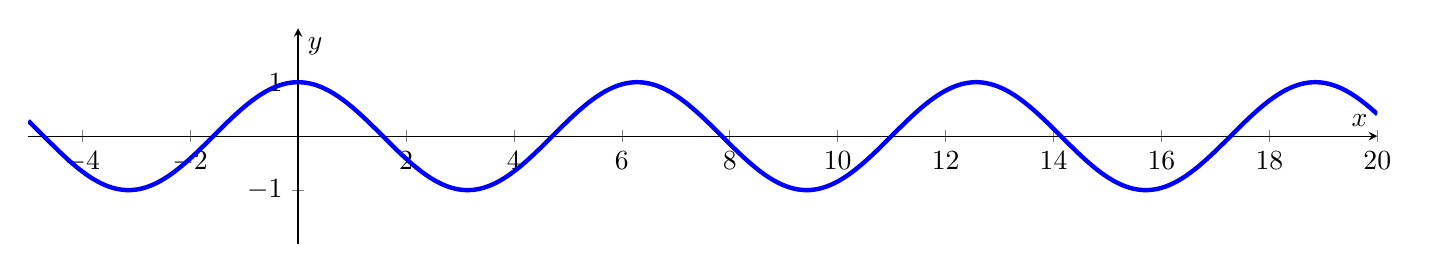
\begin{tikzpicture}
    \begin{axis}[
    scale=2.5,
    axis equal image,
    samples=500,
    axis lines=middle,
    ymin=-2,ymax=2,
    ytick={-1,1},
    ylabel=$y$, 
    xlabel=$x$
    ]
    \addplot[domain=-5:20, black, ultra thick, color=blue] {cos(deg(x))};
    \end{axis}
    \end{tikzpicture}
\end{image}
}

Remarks can simply be included in the running text, or by using \verb|\begin{remark}|:

\begin{remark}[Properties of the absolute value (with $a$ a real number)] 
		\begin{enumerate}
			\item Be careful: $|-a|= |a|$, but \textit{definitely not} $\xcancel{|-a|=a}$

			$|-a|=a$ is \textsc{incorrect} if $a<0$. Indeed, if $a=-7$, then $|-a| = |-(-7)| {\color{red}\neq} -7 = a$
			\item $|a^2 + 1| = a^2 + 1$, because $a^2+1$ is always positive.
			% \item $|a^2 - 1| = ....$ \qquad(there is \textsc{no} simple general formula without $|\cdot|$)
\end{enumerate}
\end{remark}

Examples use \verb|\begin{example}|. 
By default, examples also provide the correct answer in the handout version, while that is not the case for the exercises.

% \renewcommand{\choiceminimumverticalsize}{\vphantom{$\sqrt{2}$}} 

\begin{example}[Simple examples of absolute values]

%\begin{xmmulticols}
		\begin{enumerate}
			\item $|5|=5$ and $|-5|=5$
			\item $|\sqrt{2}-1| = $\wordChoice{\choice[correct]{$\sqrt{2} - 1$}\choice{$1-\sqrt{2}$}}
			\item $|1-\sqrt{2}| = $\wordChoice{\choice[correct]{$\sqrt{2} - 1$}\choice{$1-\sqrt{2}$}}
			\item $|2-\sqrt{2}| = $\wordChoice{\choice{$\sqrt{2} - 2$}\choice[correct]{$2-\sqrt{2}$}}
		\end{enumerate}
%\end{xmmulticols}
\end{example}






\end{document}